\chapter{Návrh systémov}\label{navrh}
Celý systém vychádza a je postavený na existujúcej platforme \emph{ACADA} cloud riešenia \emph{iTemp\footnote{Dostupnej na \url{https://www.logimic.com/itemp/}.}} vytvorenej firmou \emph{Logimic}, ktorej činnosť je opísaná v~podkapitole \ref{Logimic}.
Okrem návrhu nových funkcionalít, riešení a modelov, ktoré prináša táto bakalárska práca, sú v~následujúcich kapitolách spomenuté aj už existujúce riešenia, vzory a modely riešenia \emph{iTemp}. 
V~podkapitole \ref{navrh-architektura} je vysvetlený jednoduchý koncept riešenia. 
V~nasledujúcej podkapitole~\ref{navrh-datamodel} je navrhnutý dátový model, ktorý by bol dostačujúci pre riešenie tejto bakalárskej práce.


\section{Architektúra}\label{navrh-architektura}
Na obrázku \ref{fig:designedArch}, je vidieť veľmi zjedodušený návrh zloženia architektúry. Vidno na ňom niekoľko komponentov, kde každý spĺňa určitú úlohu. Konkrétne z~prava do ľava:\begin{itemize}
    \item \textbf{\emph{Regulátor}} je \emph{IoT} zariadenie, ktoré dokáže prijímať rádiové signály a na zákade inštrukcií z~nich ovládať výkon vykurovacieho telesa.
    \item \textbf{\emph{Teplomer}} je tiež \emph{IoT} zariadenie, ktoré ale dokáže rádiovými signálmi odosielať na~ňom namerané dáta a teda v~tomto prípade najmä teplotu vzduchu v~miestnosti kde sa nachádza.
    \item \textbf{\emph{Brána}} je taktiež \emph{IoT} zariadením, ktoré fuguje ako most medzi koncovými zariadeniami a backendovým serverom. Mení internetovú komunikáciu na rádiovú a opačne.
    \item \textbf{\emph{Sieťový server}} monitoruje, spravuje a prijíma dáta od zariadení, ktoré upravuje do~lepšie spracovateľných tvarov alebo opačne do tvarov, ktorým dané \emph{IoT} zariadenia rozumejú.
    \item \textbf{\emph{Databáza}} je organizovaná kolekcie nazbieraných dát od zariadení pre vyobrazenie daných dát ale aj nastavenia regulátora a dáta pre obslúženie ďalších služieb.
    \item \textbf{\emph{Cyklická služba}} je v~podstate program, ktorý sa vykonáva nad databázov buď v~naplánovanom čase alebo ako reakcia na napríklad príchod nového nastavenia regulátora. 
    \item \textbf{\emph{Užívateľské rozhranie}} odkazuje na vizuálnu reprezentáciu nazbieraných dát od~zariadení a poskytuje grafické prostredie pre ovládanie týchto zariadení.
\end{itemize}
\begin{figure}[h!]
    \centering
    \includesvg[inkscapelatex=false,width=0.9\columnwidth]{obrazky-figures/arch_navrh.svg}
    \caption{Návrh architektúry inteligentného kúrenia.}
    \label{fig:designedArch}
\end{figure}
\section{Dátový model}\label{navrh-datamodel}
Návrh dátového modelu je na základe zjednodušeného použitia aplikácie, pri sústredení sa na riešenie inteligentnej regulácie kúrenia. Ten je možné vidieť na obrázku \ref{fig:designedModel}.
V~tomto dátovom modeli máme entitu \emph{zariadenie} s~niekoľkými atribútmi ako jeho \emph{ID}, meno, lokáciu a typ zariadenia, z~ktorého získava ďalšie parametre a príkazy. 
Každé zariadenie patrí do miestnosti, ktorú spravuje, teda meria teplotu a ovláda kúrenie. Každá miestnosť patrí pod určitý systém. 
Ten je zas vlastnený užívateľom, ktorý zariadenia, miestnosti a systémy ďalej spravuje. 
Periodicky je cyklickou službou spomenutou v~podkapitole \ref{navrh-architektura} vytvaraný pre jednotlivé zariadenia záznam s~časovou známkou. 
Tieto záznamy slúžia napríklad na vykreslovanie grafov. 
A~tak isto sú ich parametre na základe typu zariadenia, ku ktorému daný záznam patrí.
\begin{figure}[h!]
    \centering
    \includesvg[inkscapelatex=false,width=1\columnwidth]{obrazky-figures/data_model.svg}
    \caption{Návrh datového modelu inteligentného kúrenia.}
    \label{fig:designedModel}
\end{figure}
\section{Algoritmus inteligentného  kúrenia}\label{navrh-algo}
Logika algoritmu je ukrytá v~cyklickej službe, ktorá je opísaná v~podkapitole \ref{navrh-architektura}. 
Spočíva v~troch kontrolných krokoch, či sa vôbec výpočet nového stavu spustí. Podľa diagramu z~obrázka \ref{fig:ProportionalAlgLogic} ide vyčítať nasledovné tri rozhodovacie podmienky:
\begin{itemize}
    \item \textbf{Je rozdiel nameranej teploty a nastavenej teploty významný?} Znamená to, že v~prípade ak teplota kolísa v~rozmedzí 1°C podľa zdroja \cite{TemperatureSensivity}, človek nerozlíši rozdiel. 
    Pre ušetrenie zdrojov a pre dosiahnutie čo najmenšieho počtu otvárania a zatvárania ventilu je táto hranica reflektovaná aj v~logike algoritmu ale úrovňou 0,2°C. 
    V~prípade, že rozdiel nameranej a nastavenej teda cieľovej teploty je vyšší ako tepelná sensivita človeka vyhodnotí sa podmienka ako kladná a presunie sa k~ďalšej. 
    \item \textbf{Je ich rozdiel vyšší ako nastavený kritický limit?} Myslí sa tým rozdiel nameranej a nastavenej teploty. 
    V~prípade, že tento rozdiel prekročí kritický limit je potrebné zvýšiť rýchlosť vykurovania a teda otvárať ventil rýchlejšie. To sa pri kladnej odpovedi na túto otázku prejaví ako využitie vyššieho koeficientu pri výpočte otvorenia motora. Tento koeficient je opísany ďalej v~odseku o~výpočte otvorení motora.
    \item \textbf{Pohla sa nameraná teplota požadovaným smerom od poslednej kontroly?} Hlavica sa môže nachádzať v~dvoch stavoch a to kúrenia alebo chladenia. 
    Do týchto stavov sa dostáva na základe nameraných teplôt z~minulých cyklov. 
    To znamená, že ak je hlavica v~stave kúrenia a nameraná teplota z~predošlého cyklu je stále vyššia ako práve nameraná, je nutné prepočítať otvorenie motora podľa vzorca \ref{eq:MPcalculation}.
    V~opačnom prípade ak sa teplotá zdvíha znamená to, že sa blížime k~požadovanej teplote a nieje nutné prepočítavať otvorenie motora.
\end{itemize}
\begin{figure}[H]
    \centering
    %\includesvg[inkscapelatex=false,width=0.65\columnwidth]{obrazky-figures/Algo (4).svg}
    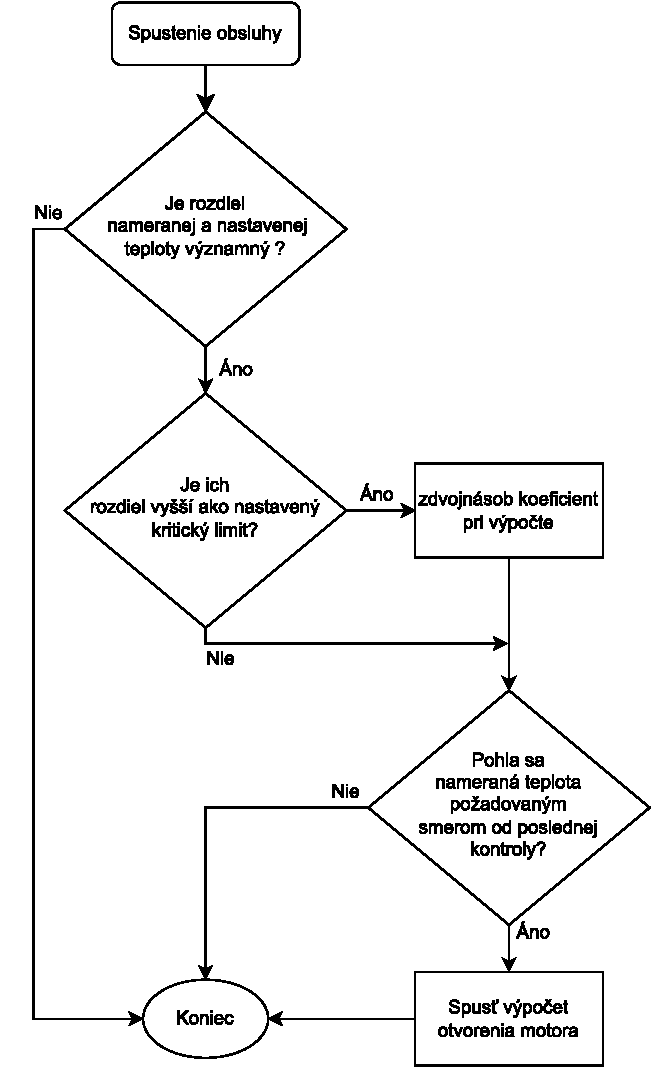
\includegraphics[width=0.65\columnwidth]{obrazky-figures/Algo (4).pdf}
    \caption{Logika inteligentného vykurovania.}
    \label{fig:ProportionalAlgLogic}
\end{figure}
\subsection*{Výpočet otvorenia motora}
Podľa následujucého vzorca \ref{eq:MPcalculation} je možné vypočítať nové otvorenia motora. 
Maximálny rozsah otvorenia motora hlavice Vicki je 0 až 800 krokov, tento rozsah sa nasledne mení podľa typu ventilu. 
Pre optimálne fungovanie hlavice je nutné zaručiť, že minimalný skok je 17 krokov inak je možné poškodenie motoru. 
Pre kalibráciu výpočtu pre miestnosti rôznych vlastností je možné použiť koeficient miestnosti v~rozsahu 0-20. 
Pre očakávané chovanie je potrebné dodržať, že cieľová teplota nesmie byť menšia ako 0.
\begin{equation}
    \centering
    \label{eq:MPcalculation}
    MP_{new} = MP_{old} - \frac{c * (T_{target} - T_{measured})*{MR}}{100}, \text{kde:}
 \end{equation}
 $MP_{new} =$ Nová pozícia motora,\\
$MP_{old} =$ Doterajšia pozícia motora,\\
$c = $ koeficient miestnosti,\\
$T_{target} = $ Cieľová teplota,\\
$T_{measured} = $ Nameraná teplota,\\
$MR = $ Maximálny rozsah motora v~krokoch,\\
\section{Komunikácia}\label{navrh-komunikacia}
Táto podkapitola sa venuje návrhu spôsobu komunikácie medzi jednotlivými komponentami z~kapitoly \ref{navrh-architektura} obrázka \ref{fig:designedArch}. Na najnižšej části, teda v~části komunikácie medzi \emph{IoT} zariadeniami, navrhujem využiť služby bezdrátového \emph{LoRaWAN} protokolu. 
Tieto zariadenia, konkrétne teda spomínaný \emph{regulátor}, \emph{teplomer} a \emph{brána} si medzi sebou budú vymieňať \emph{LoRaWAN dátové rámce}. Brána LoRa rádiové signály dešifruje a prepošle na LoRaWAN sieťový server štadartným sieťovým protokolom \emph{UDP} alebo \emph{MQTT\footnote{Viac informácii o~tomto protokole na \url{https://mqtt.org}.}}. 
Server užitočné dáta od zariadení prijíma zašifrované v~kódovaní \emph{BASE64}. 
To musí dekódovať, v~tomto prípade do hexadecimálneho kódovania. K~nemu na základe dokumentácie \emph{regulátoru} a \emph{teplomeru} je potrebné vytvoriť dekóder pre prichádzajúce správy od zariadení a kóder pre správy smerujúce na zariadenia. 
Výstupom dekódera a teda aj vstupom kódera je správa vo formáte \emph{JSON\footnote{Viac informácii o~tomto formáte na \url{https://www.json.org/json-en.html}.}.}
Táto správa je cez \emph{MQTT} poslaná ďalej na databázu, kde je správa spracovaná a uložená do databázy. 
Nad databázov bude bežať \emph{cyklická služba} s~priamým prístupom do databázy. Užívateľská aplikácia pristupuje k~databáze cez \emph{REST-API}.

\section{Užívateľské rozhranie}
Riešenie užívateľského prostredia je poskytnuté existujúcim riešením \emph{iTemp}.
Riešenie spočíva v~trojvrstvom modeli, kde s~vyššou vrstvou zachádzame do vyšších detailov. Vrstvy sú následovné:
\begin{itemize}
    \item \textbf{Layer 1} (L1), alebo prvá vrstva. Táto vrstva uchováva nastavené skupiny, kde vyobrazuje \textit{kľúčové ukazatele výkonnosti} (KPI) \cite{eckerson2010performance}. Pre užívateľskú prívetivosť sú reprezentované ako farebné štvrť kružnice okolo obrázka reprezentujúceho danú skupinu, v~tomto prípade miestnosť. Farbou sa označuje situácia v~akej sa skupina nachádza. Dané situácie sa dajú nastaviť podmienkami v~nastaveniach KPI.
    \item \textbf{Layer 2} (L2), alebo druhá vrstva ponúka bližší detail na danú skupinu s~vyšším detailom na KPI, dôležité parametry skupiny, príkazy volané nad skupinou a konkrétne zariadenia priradené do tejto skupiny.
    \item \textbf{Layer 3} (L3), alebo tretia vrstva. V~poslednej vrstve máme konkrétne zariadenia, ktoré majú detail s~väčšinou dôležitých informácii, majú svoj profil obsahujúci ich aktuálne parametre, aktívne upozornenia z~KPI, dokumentáciu o~zariadení, poslednú správu ktoré zariadenie poslalo na server, konkrétne parametre s~možnosťou editácie a nakoniec štatistiku parametrov zobrazenú v~grafoch.
\end{itemize}